%% SECTION HEADER /////////////////////////////////////////////////////////////////////////////////////
\section{Validation of the \acs{pzt} model}
\label{sec:pztVal}

%% SECTION CONTENT ////////////////////////////////////////////////////////////////////////////////////
The current model, i.e. the curved boundary geometry approximated with the second-order elements, is validated by comparing the transducer impedance obtained by numerical simulation with (i) analytical model and (ii) experimental results.

The impedance Z is a ratio between voltage \((\Phi)\) and current \((I)\) defined as follows:
\begin{eqnarray}
	Z = \frac{\Phi}{I} = \frac{\Phi}{i\omega Q},
	\label{eq:impedance}
\end{eqnarray}
\nomtypeG[omega_ang]{\(\omega\)}{Angular frequency}{}{\unit[per-mode = symbol]{\radian\per\second}}%
\nomtypeR[I]{\(I\)}{Electric current}{}{\unit{\ampere}}%
\nomtypeD[i]{\(i\)}{Imaginary number}{}%
\nomtypeR[z_impedance]{\(Z\)}{Impedance}{}{\unit{\ohm}}%
where \(i=\sqrt{-1}\), \(\omega\) is the angular frequency.
In the case of numerical simulation, \(\Phi\) is assumed as the 1.5-cycle Hann windowed sine pulse at carrier frequency 150 \unit{\kHz}, and \(Q\) is the charge induced on the electrode calculated by Eq. (\ref{eq:pzt_sem}).
The excitation signal has significant values in the 0-300 \unit{\kHz} frequency range, as shown in Fig.~\ref{fig:impedance}(\textbf{a}).
The simulations has been conducted according to the \ac{sem} model of the \ac{emi} which was implemented in \cite{fiborek2018time}.

The analytical model derived by Giurgiutiu \cite{giurgiutiu2009micromechatronics} is defined as:
\begin{eqnarray}
	Z = \frac{1}{i\omega C_0}\left[\left(1-k_p^2\right)+k_p^2\frac{u_r}{u_I}\right],
\end{eqnarray}
\nomtypeR[Capaci]{\(C_0\)}{Transducer free capacitance}{}{\unit{\farad}}%
\nomtypeD[kp]{\(k_p\)}{Transducer planar coupling coefficient}{}%
where \(C_0\) is the free capacitance of the sensor, \(k_p\) is the planar coupling coefficient, \(u_r\) is the displacement response, and \(u_I\) is the induced displacement.
Additionally, for comparison, the response of the \ac{sem} with curved boundary approximated by linear elements was included.
All models refer to the free transducer shown in Fig. \ref{fig:hioki}\textbf{(a)}, i.e. soldered wires and thin electrode coatings have been omitted.

\begin{figure}[H]
	\begin{center}
		\includegraphics[width=0.95\textwidth]{Chapter_6/hioki}
	\end{center}
	\caption{Setup for impedance measurement, \textbf{(a)} Hioki impedance analyser, \textbf{(b)} free \ac{pzt}, \textbf{(c)} transducer with soldered wires ready for measurements.}
	\label{fig:hioki}
\end{figure}
For experimental validation, an impedance analyzer (Hioki, IM 3570) was used to determine the electric current flowing through the transducer under the influence of applied voltage in the form of a sine signal with a variable frequency in the range of 1-300 \unit{\kHz}.
Both characteristics are used to determine the impedance according to Eq. (\ref{eq:impedance}).
The measurements were taken at room temperature and averaged 50 times to improve the signal-to-noise ratio.

\begin{figure}[H]
	\begin{center}
		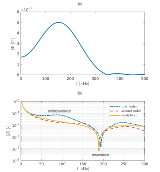
\includegraphics[width=0.95\textwidth]{Chapter_6/impedance}
	\end{center}
	\caption{Validation of the \acf{pzt} model (\textbf{a}) the frequency spectrum of the excitation signal, (\textbf{b}) impedance response of the transducer for numerical model with first order approximation of the boundary (dash-dot red line), numerical model with second order approximation of the curved boundary (dashed blue line), analytical model (dotted yellow line) and experimental measurements (solid purple line).}
	\label{fig:impedance}
\end{figure}

It can be noticed in Fig.~\ref{fig:impedance}(\textbf{b}) that the impedance of the model with second order approximation elements is in very good agreement with the analytical solution and to experimental results to the resonance peak.
The resonant peak occurred near 190 \unit{\kHz} for second order model and analytical one and 194 \unit{\kHz} in case of experimental measurement.
The model with a first-order approximation is a better fit for the experiment in frequencies above the resonant peak.
In addition, an additional antiresonance peak occurred around 90 \unit{\kHz}, which was not observed in the previous two models and analytical result.

The discrepancy in impedance based on the models and experiment may be due to uncontrolled ambient condition during the measurements and accuracy of piezo- and electromechanical properties provided by the manufacturer. 
Additionally, the models were simplified by excluding the wires and solder unlike the tested transducer shown in Fig. \ref{fig:hioki}\textbf{(b)}.